\scanpage{123}
de $i$. \deleted{\unsure{Question la structure de polarité est elle associée à} $i|\mu_2$ ?}
Donc, grâce à cette circonstance spéciale, il y a des classes de \deleted{polarité} structures polarisantes privilégiées dans $G$: les $i|\mu_2$ avec $i$ dans la classe ci-dessus.
\margin{\diagram{\begin{tikzcd}
G_{m\mathbb C}\arrow[r,dash,"i"] & G_{\mathbb C}
\end{tikzcd}}}

Quel est l'arbitraire ? On constate que l'ens \inserted{des} $(i-i'$ \deleted{\unsure{correspond à} $v_{\mathfrak p'}(\lambda)-v_{\mathfrak p}(\lambda)$} définit un sous-groupe \uline{d'indice fini} de $\operatorname{Hom}(G_{m\mathbb C},G^0_{\mathbb C})$, mais cela ne donne aucune indication sur le comportement des $i_0-i_0'$, où l'indice $0$ désigne la \unsure{restr.} à $\mu_2$. Question semble secondaire.
\margin{\diagram{\begin{tikzcd}
G_{m\mathbb C}\arrow[r,"i'"] & G_{\mathbb C}
\end{tikzcd}}}

\margin{\figure{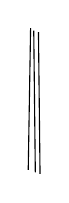
\begin{tikzpicture}
\draw (0,0)--(0.03,1.8);\draw (0.09,-0.03)--(0.07,1.77);\draw (0.15,-0.05)--(0.13,1.75);
\end{tikzpicture}}}
En tous cas, on a \deleted{des} \inserted{un} paquet de $\mathbb R$-foncteurs fibres privilégiés, définis en termes des différents $i$.

\figure{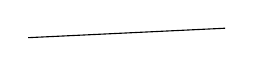
\begin{tikzpicture}\draw (0,0)--(2.5,0.12);\end{tikzpicture}}

Autre structure spécifique sur le $G$ provenant d'un corps fini: d'après la façon de l'écrire $G_{\mathbb C}:D_{\mathbb C}(M)$, $M\subset L^*$, comme $L$ est stable par conjugaison complexe, qui commute à $\operatorname{Gal}(L/Q)$, \unsure{on trouve} dans $M$ donc $G$ une involution canonique, notée
\[
u\longmapsto u'
\]
Dans $\operatorname{Ker}j^*$ c'est la symétrie, d'autre part sur $\operatorname{Im}j$ c'est l'identité, ce qui suffit pratiquement à la déterminer. Sur $\operatorname{Hom}(G_{m\mathbb C},G_{\mathbb C})$ $u\mapsto u'$ induit la conjugaison complexe.
\mspage{122}
